\documentclass[11pt]{article}
\usepackage{jheppub}
\bibliographystyle{JHEP}

\title{A comparison of sampling algorithms for particle astrophysics applications}
\author{The DarkMachines High Dimensional Sampling group: ...}
\abstract{To be abstracted.}
\keywords{Sampling, Dark Matter}
\begin{document}
\section{Introduction}
\maketitle

The core of the scientific method in the physical sciences is the extraction of the parameters of theories that can explain a variety of observations. In the modern era, the increasing size of observed datasets, combined with the increasing complexity of physical theories, has introduced a substantial computational complexity in the elucidation of correct physical theories. This is exacerbated by the fact that we have passed the era where one experiment is likely to unambiguously determine the next theory of particle physics or cosmology, and we must instead combine clues from many different branches of observation. At the same time, one can argue that substantial increases in computing power have made scientists more ambitious in the scope of both the observations and the theoretical calculations that can be used to describe the physical world.

It is often true that one can define a likelihood for a set of model parameters by, for example, simulating the results of a variety of observations, and using standard statistics to define the likelihood terms that result from each individual experiment. These can then be combined into a composite likelihood, and one can use this along with a Bayesian or frequentist statistical framework to define and obtain the ``best'' set of parameters of a given model, and the associated uncertainties. One can also use the same approach to perform model comparison. The difficulty is that the likelihood function is rarely known analytically, and can only be obtained by sampling. The simplest approach of naive random sampling is deficient for two reasons. Firstly, it is known to concentrate samples at the boundary of the space once the number of parameters is moderately large, leading to biased inferences. Secondly, it is highly inefficient in most physical examples, in which the high likelihood regions of the parameter space usually occupy a very small region of the total multidimensional volume. The past decades have thus seen the development of a series of novel sampling procedures, many of which have been utilised in particle astrophyics applications {\bf (MJW: Need a citation strategy here. I suggest a very generous citation of both the original techniques and particle astrophysics global fits that have used them)}. 

The purpose of this paper is to survey a wide range of techniques that, to the best of our knowledge, have not received mainstream use in particle astrophysics applications. We provide both a brief review of the new techniques that we have identified, and a detailed comparison of their performace with respect to each other, and to established techniques, on a range of test functions. We also attempt to optimise each technique, and provide guidelines for best practise in the field. We use both analytic test functions (for which the answer is well-known), and a physical example based on {\bf (MJW: need to choose and document this. Scalar singlet to allow for easy comparison to ScannerBit paper?)}. Real-world examples differ greatly in their challenges, depending on factors such as whether the target function is unimodal or multimodal, how expensive the likelihood function is to evaluate (which may strongly limit the number of total likelihood evaluations that can reasonably be performed), and how many nuisance parameters must be explored at the same time as the physical parameters. In the following, we attempt to provide guidance on which sort of problem might be solvable by each technique. Our ultimate aim is to provide a self-contained reference for sampling that can be used as a manual for busy particle astrophysicists, and to this end we provide a python framework with interfaces to each of the techniques described in this paper.

This paper is structured as follows. In Section~\ref{sec:algorithms}, we provide a description of each of the techniques used in this paper. In Section~\ref{sec:metrics}, we describe the metrics that we will use to compare sampler performance, for both frequentist and Bayesian applications. We provide results of comparisons on test functions in Section~\ref{sec:test}, and on a physical example in Section~\ref{sec:physics}. Finally, we present conclusions in Section~\ref{sec:conclusions}, and describe our python framework for implementing the scanning techniques described in this paper in Appendix~\ref{app:python}.

\section{Algorithms}
\label{sec:algorithms}

\subsection{Differential evolution}

\subsection{Particle swarm optimization}
\emph{Author: Pat Scott}

\subsection{Bayesian Optimization}

\emph{Author: Martin White, Zachary Searle}

\subsection{CMA evolution}
\emph{Author: Gulli Johannesson}

\subsection{AVO (population)}
\emph{Author: Joeri Hermans}

\subsection{AMPGO}
\emph{Author: Luc and Roberto} 

\subsection{Active learning}
\emph{Author: Bob Stienen}

\subsection{Nested sampling and pyBAMBI}
%\printinunitsof{in}\prntlen{\textwidth}

\emph{Author: Will Handley}
\begin{figure}
    \centerline{%
        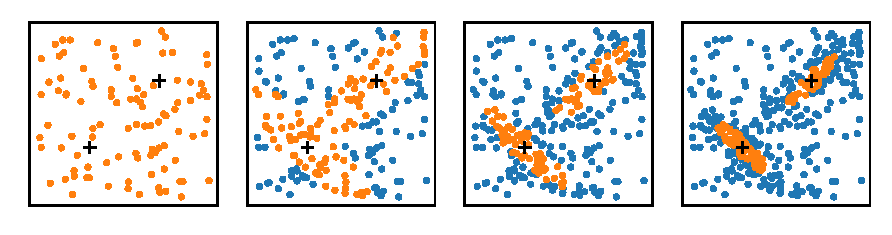
\includegraphics{nested_sampling.pdf}
    }
    \caption{Nested sampling. Live points are in orange, dead points in blue. Posterior peaks are marked with a cross.}
\end{figure}

Nested sampling~\cite{Skilling:2006gxv} is an alternative sampling strategy which simultaneously computes the Bayesian evidence whilst generating samples from the posterior distribution.
It achieves this by initially generating $n_\mathrm{live}\sim10^2-10^4$ samples from the prior. These points are then evolved these by deleting the points with the lowest likelihood, repopulating with new points drawn from the prior but at higher likelihood. The live points steadily evolve in an exponentially decreasing volume of the prior, tightening around the peak(s) of the likelihood.

The interplay between prior sampling with the likelihood entering via a constrained bound allows nested sampling to compute evidences. Furthermore, the set of discarded points may be weighted to produce posterior samples at any thermodynamic temperature, since nested sampling is an athermal algorithm~\cite{aeons}.

\texttt{PolyChord}~\cite{2015MNRAS.453.4384H,Handley:2015fda}
\texttt{MultiNest}~\cite{Feroz:2007kg,Feroz:2008xx,Feroz:2013hea}
\texttt{BAMBI}~\cite{Graff:2011gv}
\texttt{SkyNet}~\cite{Graff:2013cla}
\texttt{pyBAMBI}~\cite{pybambi}


\subsection{Sequential Neural Likelihoods}
\emph{Author: Barry Dillon}

\subsection{Calibrated approximated likelihood ratios}

\subsection{Metric Gaussian Variational Inference}
\emph{Author: Jakob Knollmueller}

\subsection{MCMC}

\emph{Author: Martin White, Csaba Balazs (Great and TWalk).} 

\section{Metrics for comparing sampling algorithms}
\label{sec:metrics}
\emph{Author: Judita Mamuzic}

\section{Comparison on test functions}
\label{sec:test}
\subsection{Frequentist}
\subsection{Bayesian}

\section{Comparison on physical example}
\label{sec:physics}
\subsection{Frequentist}
\subsection{Bayesian}

\section{Conclusions}\label{Conclusions}
\label{sec:conclusions}
\section{Acknowledgements}

\bibliography{HighDimensionalSampling}

\appendix
\section{Description of DarkMachines sampling framework}
\label{app:python}

\end{document}
